% ULaTeX2e, calling the article.cls class and 12-point type.

\documentclass[12pt]{article}

% My packages

\usepackage{amsmath}
\usepackage{framed, color}
\usepackage{soul}
\definecolor{blu}{rgb}{0,0,1}
\newcommand{\td}[1]{{\color{blu}\hl{TODO: #1}}}
\usepackage{graphicx}
\usepackage{amsthm}
\newtheorem{mydef}{Definition}
\usepackage{dcolumn}
\usepackage{multirow}
\usepackage{booktabs}
\newcolumntype{d}{D{.}{.}{4.0}}
\newcolumntype{s}{D{.}{.}{1.4}}

\usepackage{arydshln}

% Users of the {thebibliography} environment or BibTeX should use the
% scicite.sty package, downloadable from *Science* at
% www.sciencemag.org/about/authors/prep/TeX_help/ .
% This package should properly format in-text
% reference calls and reference-list numbers.

\usepackage{scicite}

% Use times if you have the font installed; otherwise, comment out the
% following line.

\usepackage{times}

% The preamble here sets up a lot of new/revised commands and
% environments.  It's annoying, but please do *not* try to strip these
% out into a separate .sty file (which could lead to the loss of some
% information when we convert the file to other formats).  Instead, keep
% them in the preamble of your main LaTeX source file.


% The following parameters seem to provide a reasonable page setup.

\topmargin 0.0cm
\oddsidemargin 0.2cm
\textwidth 16cm 
\textheight 21cm
\footskip 1.0cm


%The next command sets up an environment for the abstract to your paper.

\newenvironment{sciabstract}{%
\begin{quote} \bf}
{\end{quote}}


% If your reference list includes text notes as well as references,
% include the following line; otherwise, comment it out.

\renewcommand\refname{References and Notes}

% The following lines set up an environment for the last note in the
% reference list, which commonly includes acknowledgments of funding,
% help, etc.  It's intended for users of BibTeX or the {thebibliography}
% environment.  Users who are hand-coding their references at the end
% using a list environment such as {enumerate} can simply add another
% item at the end, and it will be numbered automatically.

\newcounter{lastnote}
\newenvironment{scilastnote}{%
\setcounter{lastnote}{\value{enumiv}}%
\addtocounter{lastnote}{+1}%
\begin{list}%
{\arabic{lastnote}.}
{\setlength{\leftmargin}{.22in}}
{\setlength{\labelsep}{.5em}}}
{\end{list}}


% Include your paper's title here

\title{Hysteresis in human computation:\\ how one task affects another} 


% Place the author information here.  Please hand-code the contact
% information and notecalls; do *not* use \footnote commands.  Let the
% author contact information appear immediately below the author names
% as shown.  We would also prefer that you don't change the type-size
% settings shown here.

\author
{Edward Newell \\ Derek Ruths\\
\\
\normalsize{\texttt{edward.newell@mail.mcgill.ca}}\\
\normalsize{\texttt{derek.ruths@mcgill.ca}}\\
\normalsize{School of Computer Science, McGill University,}\\
\normalsize{3480 University Street, Room 318, Montreal, Quebec, Canada, H3A 2A7}\\
\\
}




% Include the date command, but leave its argument blank.

\date{}



%%%%%%%%%%%%%%%%% END OF PREAMBLE %%%%%%%%%%%%%%%%



\begin{document} 

% Double-space the manuscript.

\baselineskip24pt

% Make the title.

\maketitle 



% Place your abstract within the special {sciabstract} environment.

\begin{sciabstract}
Microtask platforms have become commonplace tools for obtaining human 
annotations for large datasets.  Such platforms connect requesters 
(researchers or companies) with large populations (crowds) of workers, who 
will individually complete small information-processing jobs, each taking 
typically between one to five minutes.  
A major challenge in using such platforms, 
and a topic of ongoing research, concerns designing jobs that elicit high 
quality annotations. Here we identify a feature of nearly all crowdsourcing 
jobs that can act as a strong and systemic source of bias in annotations 
produced by workers. Specifically, many microtask jobs consist of a sequence 
of tasks which share a common format (e.g., label pictures, identify people, 
circle galaxies). Using image-labeling, a canonical microtask job format, we 
discover that earlier tasks shift the distribution of future answers by 
30-50\%. 
Moreover, we show that prior tasks influence 
the content that workers chose to focus on, as well as the richness and 
specialization of their word choice. While these intertask effects can be a 
source of systematic bias, our results suggest that, with appropriate job 
design, it might be possible to leverage these biases to hone worker focus 
and specificity, helping to elicit reproducible, expert-level judgments.
\end{sciabstract}

\section*{Main text}
Microtask platforms are online marketplaces in which \textit{requesters} 
post batches of tasks, and \textit{workers} complete them
for remuneration, a sense of purpose, and fun
\cite{kazai2013analysis,Antin20122925}.
Typical tasks include tagging and categorizing images 
\cite{6116320,Zhai2012357}, coding and transcription, such as of voice recordings or handwritten notes
\cite{chandler2013breaking,paolacci2010running,Berinsky2012351,Finnerty2013}, 
and judging relevancy and quality, for example, to rate information 
retrieval systems \cite{le2010ensuring,grady2010crowdsourcing,alonso2009can,kazai2013analysis}.

In this form of crowdsourcing, workers appear like input-output devices.  
Such platforms provide much of the flexibility and 
cost-savings of fully automating the work in a computer program: 
the workforce is available on demand over the Internet using automated 
scripts, and  no interviews or contracts are required 
\cite{wolfson2011look,5543192}.  Many tasks
can be performed at a fraction of the cost of traditional methods for 
recruiting temporary workers or experimental subjects
\cite{Berinsky2012351,paolacci2010running,ranade2012crowdsource}.
From the requester's perspective, using microtask platforms resembles
running a computer program on a remote server, leading some to investigate
these platforms as a new computing architecture \cite{5543192,little2010turkit,minder2012crowdlang,kittur2011crowdforge}.

Due to its flexibility and cost-effectiveness, 
there has been a surge in demand for microtask work
in both industry and academia\cite{wolfson2011look,Berinsky2012351}.  
Naturally, there is a desire to understand the factors affecting the 
reliability of microtask-based methods.  Researchers have investigated 
task-design parameters such as the 
level of pay \cite{Mason200977,kazai2013analysis}, 
the training and pre-screening of workers 
\cite{le2010ensuring,paolacci2010running,kazai2013analysis}, 
user-interface design \cite{Finnerty2013}, and timely feedback 
\cite{Dow20121013}.
Researchers have also investigated the effects of \textit{framing}, 
by altering the description of the workflow context 
\cite{Kinnaird2012281}, the purpose of tasks 
\cite{chandler2013breaking}, and the problem description
\cite{thibodeau2013natural}.  Another important avenue of research concerns
workflow design: how to break down a complex problem into microtasks
\cite{kittur2011crowdforge}, the effect of microtask size 
\cite{Huang201077}, and the effects of interruptions \cite{laseckieffects}.

Here, we focus on a ubiquitous feature of microtask work: the tendency
for workers to perform many similar tasks in quick succession.  
To describe this tendency, it is necessary to clarify terminology.
On one popular microtask platform, Amazon's Mechanical Turk (MTurk), 
tasks are delivered in bundles called Human Intelligence Tasks (HITs).  
But for clarity, we will use ``task'' to mean 
the smallest repeatable unit of work; for example, labeling one image with
some descriptive words (\textit{labels}).  
Using this terminology, it is typical for a HIT to
actually consist of \textit{several tasks}, 
such as labeling ten images consecutively.

In addition to the task-repetition occuring \textit{within} HITs, 
workers prefer HITs that are part of a large set of HITs
having the same format, and cite speed and repeatability 
as desireable traits \cite{Chilton20101}.  When the tasks in a sequence are 
sufficiently similar, workers are more efficient \cite{laseckieffects}, 
and the cognitive load resulting from task-switching \cite{Adamczyk2004271} 
is eliminated.  Meanwhile, breaking complex jobs down into simpler tasks 
appears to improve results \cite{kittur2011crowdforge}.  
Thus, from the perspectives of both the worker and requester, 
it is desireable for workers to perform repetitive sequences of similar 
tasks in quick succession.

The repetitive completion of tasks is of concern because people's responses
to a prompt can be strongly influenced by their recent exposure to stimuli,
due to the well-known phenomenon of \textit{priming} 
\cite{BJOP1796,No2007,beller1971priming}.  Priming is typically relevant when 
the prior stimuli bear some conceptual or perceptual connection to the 
ensuing task\cite{Gass1999549,sohn2001task}, and so, the repetition of 
similar tasks within the typical microtask setup creates an ideal context for 
strong priming effects.

Researchers investigating a somewhat similar class of psychological phenomena,
found that ratings that microtask workers give to items in a list
depend on the order in which the list is presented, an effect known as
\textit{positional bias} \cite{lerman2014leveraging}.  This serves as an 
example of a basic psychological phenomenon impacting crowdsourced data,
and raises questions about what other cognitive biases might
affect microtask work, and how prevalent the induced bias might be.  

Here we investigate the potential for task-repetition to induce bias in 
microtask-based work in a highly generalizeable setting.  
If such bias is present, it would impact virtually 
every microtask and crowdsourced workflow.
Our results show that a worker's response during a task
does indeed depend strongly on the tasks performed beforehand.   
We call the effects that earlier tasks exert on later ones 
\textit{intertask effects}.

As we have described, microtask platforms have been widely adopted as a 
tool, but computer scientists also hold such platforms as the object of 
research, viewing  microtask platforms as a new kind of computing 
architecture.  In analogy to CPUs (central 
processing units) and GPUs (graphics processing units), 
Davis \textit{et al} invoked the \textit{human processing unit}, or HPU \cite{5543192}.
Researchers have sought to define a set of basic HPU operations, and
have developed libraries and frameworks to simplify HPU programming 
and make it more like CPU programming 
\cite{little2010turkit,minder2012crowdlang,kittur2011crowdforge}.  
As an example, one operation overcomes the inherent stochasticity of HPU 
outputs, by automatically aggregating votes from multiple HPUs under a single
function call.  

But our revelation of strong intertask effects shows that, 
in addition to stochasticity, HPUs are subject to \textit{hysteresis}, 
meaning that their 
outputs depend on the history of their inputs.  Reproducibility and 
path-independence are crucial properties for the components of a 
computing architecture, so a better understanding of the computational 
ramifications of many psychological phenomena is needed. 

We investigated intertask effects using image-labeling tasks on the Amazon 
Mechanical Turk (MTurk) microtask platform.  
In addition to being one of the most common kinds of tasks
\cite{chandler2013breaking,Berinsky2012351,Finnerty2013,paolacci2010running},
image-labeling is prototypical for any kind of task in which the worker is 
asked to provide a high-level judgment, incorporating prior knowledge, in 
response to a prompt.  
This includes such diverse tasks as describing
video and audio recordings, summarizing texts, or providing feedback to a 
product review.

In our first experiment, which we call
\textit{intertask-food-objects}, workers were assigned to either a
\textit{food} or \textit{objects} treatment.  Workers in these treatments
performed a set of five \textit{initial tasks}, which each involved 
providing five descriptive labels for an image depicting 
either food or (non-food) objects, depending on the worker's 
treatment (Fig.~\ref{fig:task}A and B).  Following the initial 
tasks, workers performed five \textit{test tasks}, which were identical for 
both treatments.  The test tasks contained images depicting a 
mixture of food and objects (Fig.~\ref{fig:task}C), and workers
were again asked to provide five labels for each.  Five initial 
tasks, together with the test tasks, comprised one HIT\footnote{
	Workers were only allowed to participate in one HIT relating to this study.
}. During the HIT, workers 
were presented images one at a time, and, crucially, we made no 
distinction between the initial and test tasks.

A $\chi^2$ test shows that the frequencies of words used by
workers in the \textit{food} and \textit{objects} treatments differed
significantly during test tasks ($p = 6.0 \times 10^{-14}$), even though the test tasks were identical 
in both treatments\footnote{see supplementary text for tabulated statistics.}.  This shows that earlier tasks have a 
significant effect on later ones, and raises concerns about the 
design of microtasks, and possibly the microtask methodology itself.

While this affirms the \textit{existence} of intertask effects, we wish to
understand the nature and severity of the bias induced by prior task 
exposures.  To this end, we define the extent of bias, $\theta$, in terms of
the strength of influence that a perturbation has on worker's responses.
Since workers' responses are stochastic, we define the extent of bias in 
terms of the shift induced in the distribution of responses\footnote{
	This is a general divergence metric between probability 
	distributions known as the \textit{total variation distance.}
}:
\begin{equation}
	\theta = \frac{1}{2}\sum_{x \in X} \left| p_0(x) - p_1(x) \right|,
	\label{eq:theta}
\end{equation}
where $p_i(x)$ is the probability that a worker subjected to treatment $i$
provides response $x$, from the set of possible responses $X$.
It is important to emphasize that a significant result from a $\chi^2$ test 
only allows us to conclude that $\theta$ is non-zero 
(see supplementary text).  
Determining $\theta$ from finite samples of responses, using purely 
statistical approaches, is difficult (see supplementary text),
which leads us to reformulate the
problem in terms of classification: given a worker's 
responses to test tasks, can a machine reliably infer what her prior exposure 
had been?  Intuitively, the greater the effect that prior tasks have on 
subsequent
responses, the more accurate the classifier can be.  Formally (as shown
in the supplementary text), the accuracy of such a classifier, $\eta$,
yields a lower bound on the bias:
\begin{equation}
	\theta \geq 2\eta - 1.
	\label{l1}
\end{equation}
By measuring the accuracy of a classifier, we can bound the 
bias induced by any perturbation, including both intertask effects and 
framing.  As defined, bias ranges from 0 (meaning the exposures 
does not affect the distribution of responses), to 1 
(or 100\%) (meaning that the exposure leads workers to provide a completely
different set of responses).

\begin{figure}
	\centering
	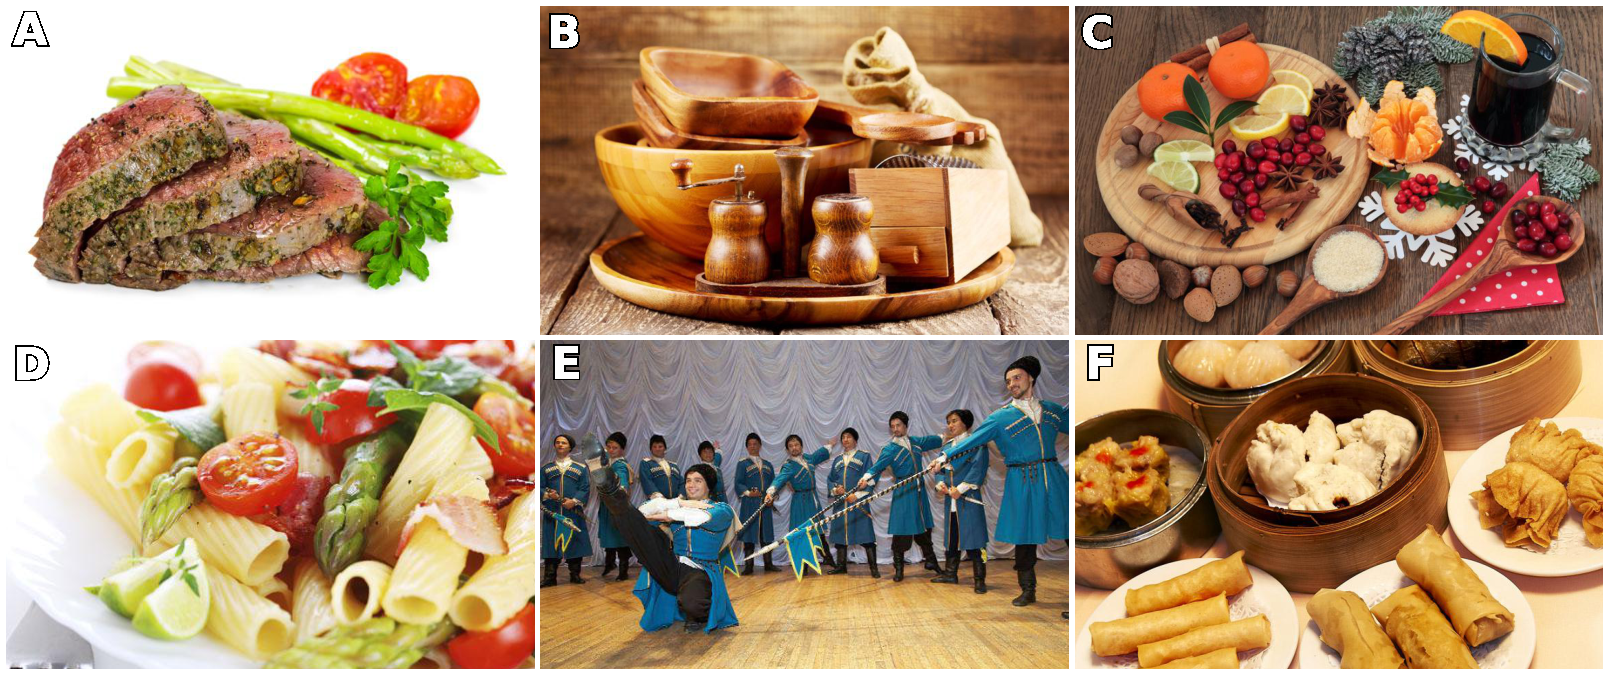
\includegraphics[scale=0.6]{figs/images.pdf}
	\caption{
		Examples of images used in
		initial tasks for the (\textbf{A}) \textit{food} and (\textbf{B}) 
		\textit{objects} treatments of \textit{intertask-food-objects};
		(\textbf{C}) test tasks for \textit{intertask-food-objects} and 
		\textit{frame-food-objects};
		initial tasks for the (\textbf{D}) \textit{food} and (\textbf{E}) 
		\textit{culture} treatments of \textit{intertask-food-culture};
		and (\textbf{F}) test tasks for \textit{intertask-food-culture} and 
		\textit{frame-food-culture}.
		The full set of experimental materials is shown in the 
		supplementary text.
	}

	\label{fig:task}
\end{figure}

Using a na\"ive Bayes classifier\footnote{
	We believe na\"ive Bayes is the best choice in this setting, as discussed
	in the supplementary material, and we show results when a support vector
	machine is used instead. 
	We also discuss data preprocessing and show results for alternatives.
}, we found that intertask effects 
lead to a 30\% bias between workers from the \textit{food} and 
\textit{objects} treatments (Fig.~\ref{fig:theta}A).  
This represents a substantial potential to distort microtask data.

There has been considerable interest in the effects that framing can have
on microtask responses
\cite{Kinnaird2012281,chandler2013breaking,thibodeau2013natural}, so,
as a point of comparison, we performed a similar experiment 
in which we framed the purpose of the tasks.  In the experiment 
\textit{frame-food-objects}, workers were either told that 
the tasks were ``Funded by the laboratory for the visual perception of Food 
and Ingredients'', or ``\ldots of Objects and Tools''.  
Framing did induce changes in the frequencies of 
word usage at significance (as determined by $\chi^2$ test; $p=0.0012$), but 
the \textit{extent} of framing-induced bias was not statistically 
distinguishable from zero ($p =0.37$) (Fig.~\ref{fig:theta}A), and was
weaker than the bias due to intertask effects ($p=2.1\times 10^{-5}$).

To assess the permenance of intertask effects, we replicated the experiment
\textit{intertask-food-objects} five times, each time using a different 
permutation of the test tasks.  This enabled us to measure the severity
of bias as a function of task position, independant of the content
of the test task.  We found that bias was strongest for the first test task
(about 28\%), but remained significant through all five test tasks 
($\alpha=0.05$) sustaining over 12\% bias (Fig. \ref{fig:theta}B).

We conducted variants of these experiments using different images, to see 
whether this trend was robust.  In the experiment 
\textit{intertask-food-culture},
workers were either assigned to a \textit{food} or \textit{culture} treatment.
As before, the initial tasks for the \textit{food} treatment contained images 
depicting food (Fig.~\ref{fig:task}D). 
In the \textit{culture} treatment, 
the initial tasks contained images depicting cultural scenes 
(of dance, sport, or music) (Fig.~\ref{fig:task}E).  The test tasks, which were identical for both
treatments, included images depicting meals of identifiable cultural 
origin\footnote{
	Despite efforts to the contrary, initial tasks 
	in \textit{intertask-food-culture} are arguably still of
	identifiable cultural origin, but this would only tend to make our 
	results more conservative (we discuss this further in the supplementary 
	text).
}
(Fig.~\ref{fig:task}F).  

Results for this experiment again showed a 
strong bias as a result of intertask effects (about 50\%) 
(Fig.~\ref{fig:theta}A).  Again, we compared intertask effects to 
framing, by performing an experiment (\textit{frame-food-culture}) using 
the same test tasks as in \textit{intertask-food-culture}, in which we exposed
workers to a statement framing the purpose of the tasks as the recognition 
of either food or culture.  
In this experiment, framing did not induce significant changes in the 
frequencies of words used during test tasks (by $\chi^2$ test, $p=0.29$) 
(Fig.~\ref{fig:theta}A).

It was only when we combined the use of framing, with an active 
reiteration step, that bias reached a level comparable to that achieved 
by intertask effects.  In the experiment \textit{echo-food-objects},
after framing the purpose of the task around either the recognition of food
or objects, we required the worker to echo back the purpose of the task
using a combo-box input.  In this case, workers exposed to different 
``echoed framing'' showed a bias of about 35\% in the labels provided during 
test tasks
(Fig.~\ref{fig:theta}A). However, it is difficult to say whether this 
should be considered as a framing treatment \textit{per se}.
Requiring the worker to reiterate the frame signals our intent, as the 
requester, to ensure that the worker has taken note of the framing statement, 
possibly leading the worker to interpret it as an instruction.  
In any case, it is remarkable that intertask effects
were on par with an explicit statement of purpose that was emphasized 
through reiteration.

\begin{figure}
	\centering
	\includegraphics[scale=1]{figs/theta.pdf}
	\caption{
		Empirical bias, $\theta_\mathrm{NB}$, measured using a na\"ive Bayes 
		classifier, induced in image labeling tasks,
		(\textbf{A}) by exposing workers to initial tasks or framing. 
		As workers proceed through test tasks, the effects of initial tasks 
		wane, as shown (\textbf{B}) for \textit{intertask-food-objects}, but 
		remain significant even after five tasks.  Standard error bars are 
		shown.
	}
	\label{fig:theta}
\end{figure}

\begin{figure}
	\centering
	\includegraphics[scale=0.92]{figs/vocab_specificity.pdf}
	\caption{
		(\textbf{A}) Exposing workers to initial tasks or framing, 
		involving food, changed the subsequent fraction of words that 
		referred to food during test tasks, 
		but did not always increase that fraction (in all three plots,
		positive values indicate a larger quantity for food-exposed workers).
		(\textbf{B}) The number of unique food-related
		words (richness) was greater for food-exposed workers, except in the 
		case of \textit{frame-food-culture} (stars indicate the threshold
		for a significant deviation under the null hypothesis of equal 
		richness, $\alpha=0.05$). 
		(\textbf{C}) Food-exposed
		workers used more specialized words to refer to food (see 
		supplementary text for calculation of relative specialization).
		Standard error bars are shown in (\textbf{A} and \textbf{C}).
	}
	\label{fig:specificity}
\end{figure}

To better understand the nature of 
intertask effects, we investigated the vocabulary
that workers used to label test tasks. A natural expectation is that, during
the test tasks within
a given experiment, the food-primed workers would use food-related words 
more often than their non-food-primed counterparts.  However, this was not 
generally 
the case. In the \textit{intertask-food-culture} experiment, food-primed
workers actually used significantly \textit{fewer} food-related words 
during test tasks\footnote{
	food-related words were identified using the wordnet corpus, 
	augmented with additional words obtained by crawling a recipe website 
	(see supplementary text for details).
} (Fig.~\ref{fig:specificity}A).  This finding
rules out a seemingly-simple idea that workers emphasize
content that has been present in earlier tasks: seeing content in prior tasks
influences, but does not necessarily \textit{increase}, the probability of 
referring to the content in subsequent tasks.

To deepen our understanding, we investigated workers' lexical richness in 
reference to food, that is, the number of \textit{unique} food-related words
used.  Even if workers provide an abundance of food-related words, there
can be less diversity if the same words are often repeated.  
This could happen, for example, if workers use generic references 
to food.
Both \textit{intertask} experiments showed that food-exposed workers had 
greater lexical richness, in reference to food, than their non-food-primed 
counterparts (as much as 20\% more) (Fig.~\ref{fig:specificity}B).  
The increase in lexical richness in the case of 
\textit{intertask-food-culture} is particularly noteworthy, because in that 
experiment, food-primed workers made fewer total references to food.  
We also observed enrichment of the food-related lexicon in the 
\textit{priming-food-objects}, and \textit{echo-food-objects} experiments, 
although to a lesser extent.

The observations regarding lexical richness lead us to suspect that 
initial tasks might influence workers to use more refined or specialized 
words, when referring to aspects of content that had been present in the 
initial tasks (i.e. food).  This would help explain why, in the case of 
\textit{intertask-food-culture}, we observed a significantly greater 
\textit{diversity} of food-related words despite their significantly lesser 
\textit{total amount}.
To test whether exposure to food in initial tasks increased the specialization
of food-references, we used the wordnet corpus to operationalize the 
notion of word specialization.  Wordnet provides a set of hypernym-hyponym 
relations between 117,798 English nouns 
\cite{miller1995wordnet,felbaum1998wordnet}.  Hypernyms are generalizations 
(for example, ``bread'' is a hypernym for 
``pumpernickel''), while hyponyms are specializations.
For each experiment, we compared food-related words provided by workers from 
one treatment to those from the other, tallying the percent-excess of
cases where one treatment's words were more specialized than the other 
(detailed calculation in the supplementary text). 

In all experiments except \textit{frame-food-culture}, food-primed workers 
used significantly more specialized words, in reference to food, 
than their non-food-primed 
counterparts (about 15\% more) (Fig.~\ref{fig:specificity}C).
It is interesting that such substantial increases in both the lexical 
richness and specialization of food-related words 
held for \textit{intertask-food-culture}, where, as mentioned, we observed 
that food-exposed workers made \textit{fewer} references to food overall. 
These observations point 
to countervailing factors: one factor tending to activate the more 
specialized and less common food-related words 
(yielding greater lexical richness and specialization), and the other tending 
to suppress certain, presumably more common and generic words 
(yielding fewer food-related words in total).

This hypothesis is corroborated when we look at those words whose 
frequencies changed the most from one treatment to another 
(Table~S\ref{table:top-words}).  
The word ``food'', which is the most generic possible food-related word, was 
always \textit{suppressed} among food-primed workers.  In fact, 
for all experiments, ``food'' was the \textit{most suppressed} word.

Taken together, our results can be 
explained through a combination of positive and negative priming effects.
Positive priming (usually simply ``priming'') occurs when a prior stimulus 
predisposes a person to give certain responses in an ensuing task, and
is often observed as an increase in the speed or accuracy of a response, or
the ability to recognize briefer or noisier stimuli 
\cite{BJOP1796,BJOP1826,Huber2008324}.
Negative priming occurs when, after exposure to a stimulus 
considered to be non-salient, subsequent recognition of the stimulus is 
inhibited \cite{mayr2007negative}.

Workers exposed to images containing food will be (positively) primed, 
activating memories, concepts, and vocabulary related to food.  
However, as the worker labels successive images containing food, the basic 
fact that an image contains food will not appear to be salient, since it 
does not serve to distinguish one image from another.  Thus, the most 
generic references to that fact, such as the label ``food'', 
will be suppressed, while more specialized references will be elicited.  
Meanwhile, the number of references to food overall might increase or 
decrease, depending on the balance of these factors.  

More generally, we are suggesting that, even though workers are not 
instructed to compare tasks in any way, prior tasks form a 
context relative to which workers judge salience.  Thus, due to a combination 
of negative and positive priming, a worker's focus 
in repeated tasks tends to be directed away from generic, shared features, 
toward specific and distinguishing ones.

Prior to this study, little thought appears to have been given to the 
priming effect that a task can have on those tasks that follow. 
But our findings show this is an  
important design consideration.  
A natural response might be simply to randomize 
task ordering, a practice that is commonly employed.  But the sheer extent of 
bias suggests that this will still introduce a significant amount of noise
into the results.  Even chains of two or three similar tasks, which
will not be reliably eliminated in random permutations, could lead
to the levels of bias we observed in our experiments.
It would be preferable to understand intertask
effects in greater depth so that they might be properly controlled.

Our findings suggest that, through careful task engineering,
it might be possible to achieve greater quality and reproducibility
of responses.  
A consistent goal in human computation is the achievement of expert-level
judgments from non-expert workers \cite{kittur2011crowdforge}.  
This has been achieved in some
applications \cite{snow2008cheap,Mortensen20131020,Warby2014385}. 
The distinction between experts and novices can be 
attributed in part to the possession of specialized knowledge and heuristics. 
But to a large degree, this distinction lies in the ability of 
experts to direct their focus toward salient features, while filtering out 
non-salient ones \cite{kellman2009perceptual}.  Using strategic task 
exposure, it might be possible to guide workers' focus and salience 
attribution, enabling expert-level judgment in a wider variety of 
crowdsourced applications.
We anticipate that future work will yield techniques to control intertask 
effects, both to reduce unwanted bias, as well as tune the 
focus, diversity, and specificity of worker responses.

Here we have shown that a severe bias can be introduced into microtask 
responses, simply from the performance of earlier tasks. 
These effects are much stronger than the effects of framing.  
While our findings raise serious concerns about the 
current state of microtask design, they reveal potential opportunities 
for more 
refined control over worker focus and acuity.  Any application that relies
on the repetitive use of human judgment is likely subject to the phenomena
we described here.  Exploring the pitfalls and opportunities posed by
intertask effects is an important direction for future work, 
in the effort to develop performant and reliable methods for human 
computation.
\bibliography{newbib}
\bibliographystyle{Science}
\end{document}


